\addcontentsline{toc}{chapter}{Занятие 1. Выборочные характеристики}
\chapter*{Занятие 1. Выборочные характеристики}

\addcontentsline{toc}{section}{Контрольные вопросы и задания}
\section*{Контрольные вопросы и задания}

\subsubsection*{Приведите определение выборки, вариационого ряда, статистики, порядковой статистики,
                эмпирической функции распределения.}

$x_1, \dotsc, x_n$ --- наблюдаемые значения ---
независимые одинаково распределённые случайные величины с неизвестной функцией распределения
$F \left( x \right) $.

Такой набор случайных величин называется выборкой из распределения $F$.

Вариационный ряд --- последовательность $x_{ \left( 1 \right) }, \dotsc, x_{ \left( n \right) }$,
полученная в результате расположения в порядке неубывания исходной последовательности
независимых одинаково распределённых случайных величин $x_1, \dotsc, x_n$.

Статистикой называют функцию $S$ от выборки $X = \left( x_1, x_2, \dotsc, x_n \right) $ такую,
что $S \left( X \right) = S \left( x_1, x_2, \dotsc, x_n \right) $.

Вариационный ряд и его члены являются порядковыми статистиками.

Эмпирической (выборочной) функцией распределения,
построенной по выборке $x_1, \dotsc, x_n$ называется функция
$$F_n \left( x \right) =
  \frac{1}{n} \sum \limits_{k = 1}^n \mathbbm{1}_{x_k \leq x}, \,
  x \in \mathbb{R}.$$

\subsubsection*{Какими свойствами обладает эмпирическая функция распределения?}

Есть множество полной вероятности,
на котором эмпирическая функция распределения аппроксимирует функцию распределения,
то есть почти наверное $F_n \Rightarrow F, \, n \to \infty $.

\subsubsection*{Запишите выражения для выборочного среднего, выборочной диспресии,
                выборочных моментов.}

$$ \frac{1}{n} \sum \limits_{k = 1}^n x_k$$
--- выборочное среднее.

Выборочная дисперсия
$$ \hat{ \sigma^2} =
  \frac{1}{n - 1} \sum \limits_{k = 1}^n \left( x_k - \overline{x} \right)^2.$$

Выборочные моменты в математической статистике ---
это оценка теоретических моментов распределения на основе выборки.

Выборочный момент порядка $k$ --- это случайная величина
$$a_n \left( k \right) =
   \frac{1}{n} \sum \limits_{i = 1}^n x_i^k.$$

\addcontentsline{toc}{section}{Аудиторные задачи}
\section*{Аудиторные задачи}

\subsubsection*{1.4}

\textit{Задание.}
Пусть $X_1, \dotsc, X_n$ ---
выборка из равномерного распределения на отрезке $ \left[0, \theta \right] $
с неизвестным параметром $ \theta $.
Какие из приведённых ниже функций являются статистиками?
\begin{enumerate}[label=\alph*)]
  \item $ \overline{X}$;
  \item $5X_{ \left( n \right) }$;
  \item $ \theta / 2$;
  \item $X_1 / \theta $;
  \item $X_{ \left( 1 \right) } + X_1 + X_n$.
\end{enumerate}

\textit{Решение.}
\begin{enumerate}[label=\alph*)]
  \item Да;
  \item да;
  \item нет, так как не функция от выборки;
  \item функция не только от выборки (зависит от неизвестного параметра).
  Отсюда следует, что это не статистика;
  \item да.
\end{enumerate}

\subsubsection*{1.5}

\textit{Задание.}
Пусть $X_1, \dotsc, X_n$ --- выборка из распределения Пуассона с параметром $ \lambda $.
Вычислите математическое ожидание и дисперсию статистики
$$ \overline{X} =
  \frac{1}{n} \sum \limits_{i = 1}^n X_i.$$
Выясните, имеет ли статистика $ \overline{X}$ распределение Пуассона.

\textit{Решение.} Все $X_i$ одинаково распределены.
Отсюда следует, что все математические ожидания одинаковы
$$M \overline{X} =
  \frac{1}{n} \sum \limits_{i = 1}^n MX_i =
  \frac{1}{n} \cdot nMX_1 =
  MX_1 =
  \lambda.$$

Для всякой выборки справедливо $M \overline{X} = MX_1$.

Из независимости $X_i$ получаем
$$D \overline{X} =
  \frac{1}{n^2} \sum \limits_{i = 1}^n DX_i.$$

Так как $X_i$ одинаково распределены, то все дисперсии одинаковы
$$D \overline{X} =
  \frac{DX_1}{n} =
  \frac{ \lambda }{n}.$$

Математическое ожидание и дисперсия для распределения Пуассона совпадают.
Отсюда следует, что эта случайная величина не имеет распределения Пуассона.

$ \overline{X}$ не обязательно буде принимать целые значения.

\subsubsection*{1.6}

\textit{Задание.} Вычислите математическое ожидание статистик:
\begin{enumerate}[label=\alph*)]
  \item $S^2 = \overline{X^2} - \left( \overline{X} \right)^2$;
  \item $S_0^2 =
          1 / \left( n - 1 \right) \cdot
          \sum \limits_{i = 1}^n \left( X_i - \overline{X} \right)^2$.
\end{enumerate}

\textit{Решение.}
\begin{enumerate}[label=\alph*)]
  \item Распишем каждую из величин
  $$S^2 =
    \overline{X^2} - \left( \overline{X} \right)^2 =
    \frac{1}{n} \sum \limits_{i = 1}^n X_i^2 -
    \left( \frac{1}{n} \sum \limits_{i = 1}^n X_i \right)^2.$$
  Распишем квадрат
  $$ \frac{1}{n} \sum \limits_{i = 1}^n X_i^2 -
    \left( \frac{1}{n} \sum \limits_{i = 1}^n X_i \right)^2
    \frac{1}{n} \sum \limits_{i = 1}^n X_i^2 -
    \frac{1}{n^2} \left(
      \sum \limits_{i = 1}^n X_i^2 + 2 \sum \limits_{i, j = 1, i < j}^n X_i X_j
    \right).$$
  Берём слева и справа математическое ожидание.
  Из того, что случайные величины в выборке одинаково распределены
  $$MS^2 =
    MX_1^2 - \frac{1}{n^2} \left[ nMX_1 + 2C_n^2 \left( MX_1 \right)^2 \right].$$
  Подставляем $C_n^2$ и группируем
  $$MX_1^2 - \frac{1}{n^2} \left[ nMX_1 + 2C_n^2 \left( MX_1 \right)^2 \right] =
    \frac{n - 1}{n} \cdot MX_1^2 - \frac{n - 1}{n} \left( MX_1 \right)^2.$$
  Вынесем общий множитель за скобки
  $$ \frac{n - 1}{n} \cdot MX_1^2 - \frac{n - 1}{n} \left( MX_1 \right)^2 =
    \frac{n - 1}{n} \left[ MX_1^2 - \left( MX_1 \right)^2 \right] =
    \frac{n - 1}{n} \cdot SX_1.$$
  Эта оценка смещена ассимптотически;
  \item выразим $S_0$ через $S$.
  Раскроем квадрат
  $$S_0^2 =
    \frac{1}{n - 1} \sum \limits_{i = 1}^n \left( X_i - \overline{X} \right)^2 =
    \frac{1}{n - 1}
    \sum \limits_{i = 1}^n \left( X_i^2 - 2X_i \overline{X} + \overline{X}^2 \right).$$
  Имеем сумму $n$ одинаковых слагаемых
  $$ S_0^2 =
    \frac{1}{n - 1}
    \left( n \overline{X^2} - 2 \left( \overline{X} \right)^2 n + n \overline{X}^2 \right) =
    \frac{n}{n - 1} \left[ \overline{X^2} - \left( \overline{X} \right)^2 \right] =
    \frac{n - 1}{n} \cdot S^2.$$
  Отсюда следует, что
  $$MS_0^2 =
    \frac{n}{n - 1} \cdot \frac{n - 1}{n} \cdot DX_1 =
    DX_1.$$
\end{enumerate}

\subsubsection*{1.7}

\textit{Задание.} Найдите в терминах функции распределения $F$ выборки $X_1, \dotsc, X_n$:
\begin{enumerate}[label=\alph*)]
  \item распределение $k$-ой порядковой статистики $X_{ \left( k \right) }$;
  \item вероятность
  $P \left( X_{ \left( k \right) } < y, \, X_{ \left( k + 1 \right) } \geq y \right) $.
\end{enumerate}

\textit{Решение.}
\begin{enumerate}[label=\alph*)]
  \item Сделали упорядочивание случайных величин
  $$X_{ \left( 1 \right) } \leq
    X_{ \left( 2 \right) } \leq
    \dotsc \leq
    X_{ \left( k \right) } \leq
    \dotsc \leq
    X_{ \left( n \right)}.$$

  По определению
  $F_{X_{ \left( k \right) }} \left( y \right) =
    P \left( X_{ \left( k \right) } \leq y \right) =
    P$\{хотя бы $k$ элементов выборки не превышает $y$\} =
  $$= \sum \limits_{i = k}^n P(A_i),$$
  где $A_i =$ \{ровно $i$ элементов выборки не превышают $y$\}.

  Есть $n$ испытаний, успех --- $X_i \leq y$.

  Вероятность успеха --- это $F \left( y \right) $, вероятность неудачи ---
  это $ \left[ 1 - F \left( y \right) \right] $.
  Это биномиальное распределение
  $$F_{X_{ \left( k \right) }} =
    \sum \limits_{i = k}^n
      C_n^i F^i \left( y \right) \left[ 1 - F \left( y \right) \right]^{n - i};$$
  \item согласно с предыдущим пунктом
  $P \left( X_{ \left( k \right) } < y, \, X_{ \left( k + 1 \right) } \geq y \right) =
    P$\{ровно $i$ элементов выборки не превышает $y$\} $=
    C_n^k F^k \left( y \right) \left[ 1 - F \left( y \right) \right]^{n - k}$.
\end{enumerate}

\subsubsection*{1.8}

\textit{Задание.}
Пусть $ \left( -0.8; 2.9; 4.5; -5.7; 1.1; -3.2 \right) $ --- наблюдаемые значения выборки.
Составьте вариационный ряд,
постройте эмпирическую функцию распределения $F_6 \left( x \right) $ и её график.
Вычислите выборочное среднее и выборочную дисперсию.

\textit{Решение.} Вариационный ряд: $ \left( -5.7; -3.2; -0.8; 1.1; 2.9; 4.3 \right) $.

Эмпирическая функция распределения (рис. \ref{fig:18}).
$$F_6 \left( y \right) =
  \frac{1}{6} \sum \limits_{i = 1}^6 \mathbbm{1} \left\{ x_i \leq y \right\} =
  \begin{cases}
    0, \qquad x < -5.7; \\
    \frac{1}{6}, \qquad -5.7 \leq x < -3.2, \\
    \frac{2}{6}, \qquad -3.2 \leq x < -0.8, \\
    \frac{3}{6}, \qquad -0.8 \leq x < 1.1, \\
    \frac{4}{6}, \qquad 1.1 \leq x < 2.9, \\
    \frac{5}{6}, \qquad 2.9 \leq x < 4.3, \\
    1, \qquad x \geq 4.3.
  \end{cases}$$

\begin{figure}[h!]
  \centering
  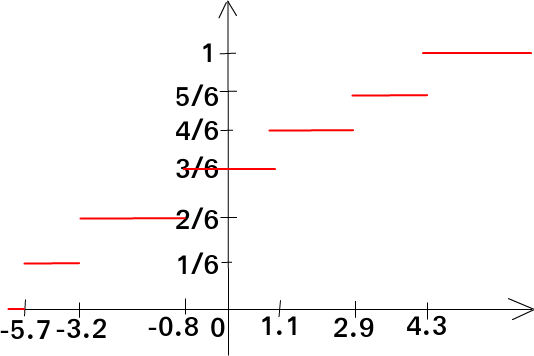
\includegraphics[width=.4\textwidth]{./pictures/1_8.png}
  \caption{Эмпирическая функция распределения}
  \label{fig:18}
\end{figure}

Выборочное среднее
$$ \overline{X} =
  \frac{1}{6} \left( -5.7 -3.2 - 0.8 + 1.1 + 2.9 + 4.3 \right) =
  \frac{1}{6} \left( -9.7 + 8.3 \right) =
  - \frac{1}{6} \cdot 1.4 =
  -0.23.$$

Выборочная дисперсия
$$ \hat{ \sigma }^2 =
  \frac{1}{5} \sum \limits_{i = 1}^6 \left( X_i + 0.23 \right)^2.$$
Она является несмещённой.

\subsubsection*{1.9}

\textit{Задание.}
Вычислите вероятность $P \left( F_n \left( y \right) < F_n \left( z \right) \right) $.

\textit{Решение.}
\begin{enumerate}[label=\alph*)]
  \item $y \geq z$.
  Событие невозможное, потому что $F_n \left( y \right) \geq F_n \left( z \right) $;
  \item рассмотрим случай, когда $y < z$.

  Тогда искомая вероятность равна
  $P \left( F_n \left( y \right) < F_n \left( z \right) \right) = P$
  \{в $ \left( y, z \right) $ попал хотя бы 1 элемент выборки\}
  $= 1 - P$\{в $ \left( y, z \right) $ ни один элемент выборки не попал\}.
  Случайные величины одинаково распределены,
  поэтому $1 - P$\{в $ \left( y, z \right) $ ни один элемент выборки не попал\} $= \\
  = \left[ 1 - P \left\{ x_i \notin \left( y, z \right) \right\} \right]^n =
  1 - \left[ 1 - P \left\{ x_1 \in \left( y, z \right) \right\} \right]^n = \\
  = 1 - \left[ 1 - P \left( x_1 < z \right) + P \left( x_1 < y \right) \right]^n =
  1 - \left[ 1 - F \left( z \right) + F \left( y \right) \right]^n$.
\end{enumerate}

\addcontentsline{toc}{section}{Домашнее задание}
\section*{Домашнее задание}

\subsubsection*{1.15}

\textit{Задание.}
Пусть $X_1, \dotsc, X_n$ ---
выборка из равномерного на отрезке $ \left[ a, b \right] $ распределения.
Вычислите математическое ожидание и дисперсию статистики
$$ \overline{X} =
  \frac{1}{n} \sum \limits_{i = 1}^n X_i.$$
Выясните, имеет ли статистика $ \overline{X}$ равномерное распределение; нормальное распределение.

\textit{Решение.} Все $X_i$ одинаково распределены.
Отсюда следует, что все математические ожидания одинаковы
$$M \overline{X} =
  \frac{1}{n} \sum \limits_{i = 1}^n MX_i =
  \frac{1}{n} \cdot nMX_1 =
  MX_1 =
  \frac{a+b}{2}.$$

Из независимости $X_i$ получаем
$$D \overline{X} =
  \frac{1}{n^2} \sum \limits_{i = 1}^n DX_i.$$

Так как $X_i$ одинаково распределены, то все дисперсии одинаковы
$$D \overline{X} =
  \frac{DX_1}{n} =
  \frac{ \left( b - a \right)^2}{12n}.$$

Чтобы выяснить,
распределена ли статистика $ \overline{X}$ по нормальному или равномерному распределению,
найдём её характеристическую функцию $ \varphi_{ \overline{X}} \left( t \right) $.
Учитывая независимость элементов выборки и то, что
$$ \varphi_{X_1} \left( t \right) =
  \dotsc =
  \varphi_{X_n} \left( t \right) =
  \frac{e^{itb} - e^{ita}}{it \left( b - a \right) },$$
находим
$$ \varphi_{ \overline{X}} \left( t \right) =
  \varphi_{X_1} \left( \frac{t}{n} \right) \cdot
  \dotsc \cdot
  \varphi_{X_n} \left( \frac{t}{n} \right) =
  \left[ \frac{\left( e^{itb} - e^{ita} \right) n}{it \left( b - a \right)} \right]^n.$$
Отсюда следует, что $ \overline{X}$ не имеет указанных распределений.

\subsubsection*{1.16}

\textit{Задание.}
Пусть $X_1, \dotsc, X_n$ --- выборка из некоторого распределения вероятностей,
функция распределения которого $F$ является непрерывной и строго возрастающей.
Найдите распределение выборки $Y_1, \dotsc, Y_n$, где
$$Y_i =
  F \left( X_i \right).$$

\textit{Решение.}
По определению
$$F_{ \eta_1, \dotsc, \eta_n} \left( X_1, \dotsc, X_n \right) =
  P \left( \eta_1 \leq X_1, \dotsc, \eta_n \leq X_n \right).$$
Воспользуемся независимостью
$$P \left( \eta_1 \leq X_1, \dotsc, \eta_n \leq X_n \right) =
  P \left( \eta_1 \leq X_1 \right) \cdot \dotsc \cdot P \left( \eta_n \leq X_n \right).$$

Функция распределения $i$-й компоненты вектора равна
$$F_{ \eta_i} \left( x \right) =
  P \left( F_{ \xi_i} \left( X_i \right) \leq x \right) =
  \begin{cases}
    0, \qquad x \leq 0, \\
    1, \qquad x > 1.
  \end{cases}$$

Рассмотрим $ \left[ 0, 1 \right] $.

Поскольку $F$ --- непрерывная и строго возрастающая, то существует $F^{-1} \left( x \right) $.
Обозначим через $z$ точку $F^{-1} \left( x \right) $ такую, что $F \left( z \right) = x$.
Событие $ \left\{ \eta = F \left( \xi \right) < x \right\} $ происходит тогда и только тогда,
когда происходит событие $ \left\{ \xi < z \right\} $.

Получаем на отрезке $ \left[ 0, 1 \right] $ равномерное распределение
$$F_{ \eta } \left( x \right) =
  F_{ \xi } \left( z \right) =
  F_{ \xi } \left( F_{ \xi }^{-1} \left( x \right) \right) =
  \begin{cases}
    0, \qquad x \leq 0, \\
    x, \qquad x \in \left( 0, 1 \right] ,\\
    1, \qquad x > 1.
  \end{cases}$$
